\documentclass{article}
\usepackage[utf8]{inputenc}
\usepackage[T1]{polski}
\usepackage{graphicx}
\usepackage{float}
\usepackage{geometry}
\geometry{left=20mm, right = 20mm, bottom=20mm}

\title{Specyfikacja implementacyjna programu Karetki W Pogotowiu}
\author{Karolina Czachorska, Adrian Milewski, Bartłomiej Anczok, Maxymilian Kowalski}
\date{\today}

\begin{document}

\maketitle

\tableofcontents
\newpage

\section{Cel dokumentu}
Dokument ten jest specyfikacją implementacyjną dla programu Karetki W Pogotowiu. Opisane będzie środowisko deweloperskie, zasady wersjonowania, diagram i opis klas oraz opis głównych algorytmów.\\
\section{Środowisko deweloperskie}
\subsection{Język programowania}
Program będzie tworzony w języku Java, w wersji 15.\\
\subsection{Zintegrowane środowisko programistyczne}
Karetki W Pogotowiu będą tworzone z wykorzystaniem środowisk IntelliJ IDEA Ultimate i Apache Netbeans IDE.\\
\section{Zasady wersjonowania}
\subsection{Wpisy do repozytorium}
Wpisy do repozytorium będą tworzone w języku angielskim. W zależności od etapu pracy będą one miały przedrostki:\\
\begin{itemize}
\item \textit{in progress:} - jeżeli dana funkcjonalność nie będzie jeszcze skończona,
\item \textit{to test:} - jeżeli dana funkcjonalność będzie musiała zostać przetestowana,
\item \textit{done:} - jeżeli dana funkcjonalność będzie już skończona.
\end{itemize}

\subsection{Gałęzie}
Każda grupa funkcjonalności będzie tworzona z wykorzystaniem oddzielnej gałęzi:
\begin{itemize}
\item Odczyt i walidacja pliku - gałąź \(input-file-read\)
\item Określenie granic kraju oraz położenia pacjentów względem niego - gałąź \(convex-hull\)
\item Obsługa transportu pacjenta do szpitala - gałąź \(transport-patient\)
\item Graficzny interfejs użytkownika - gałąź \(GUI\)
\item Zapis wyniku do pliku / wypisywanie wyniku działania programu - gałąź \(output\)
\end{itemize}
Po zakończeniu pracy nad daną funkcjonalnością zostanie ona dołączona do gałęzi master. Jeżeli zajdzie potrzeba dodania zmian lub naprawienia błędów w kodzie znajdującym się w gałęzi master to stworzona zostanie oddzielna gałąź o nazwie \(FIX:<issue>\), gdzie \(issue\) to problem wymagający naprawy.

\section{Główny algorytm}
Podstawowe działanie programu można podzielić na dwie główne części:
\begin{itemize}
\item Podział szpitali i obiektów na otoczkę wypukłą i resztę punktów oraz sprawdzanie czy pacjent znajduje się w kraju (w otoczce)
\item Poruszanie się po szpitalach z pacjentem
\end{itemize}
Do rozwiązania problemów postawionych w pierwszym punkcie zastosujemy dwa algorytmy oraz kilka własności matematycznych:
\begin{enumerate}
\item \textbf{Graham's scan } jako algorytm pozwalający znaleźć otoczkę wypukłą z \textbf{\textit{N}} podanych punktów w czasie \textbf{O(\textit{NlogN})}
\item \textbf{Wyszukiwanie binarne} aby znaleźć pierwszy punkt należący do otoczki, którego kąt skierowany jest większy niż kąt punktu położenia rozpatrywanego pacjenta, a następnie sprawdzenie czy punkt leży w odpowiednim trójkącie na podstawie własności pola (jeżeli punkt leży wewnątrz trójkąta, to suma pól utworzonych między nim a bokami trójkąta będzie równa polu całego trójkąta).
\end{enumerate}
Aby rozwiązać problemy postawione w drugiej części jedyne co należy zrobić to:
\begin{enumerate}
\item Utworzyć listę sąsiedztwa dla każdego szpitala, \textbf{algorytmem dijkstry} maksymalnie skrócić wszystkie odległości w każdej liście i posortować ją względem odległości od sąsiednich szpitali,
\item Zapamiętywać czy dany szpital został odwiedzony przez danego pacjenta oraz poruszać się z pacjentem po szpitalach za pomocą wcześniej utworzonych list sąsiedztwa.
\end{enumerate}

\newpage
\section{Szczegóły implementacyjne}
\subsection{Diagram klas}
Na poniższym diagramie przedstawione zostały główne klasy, które będą używane podczas tworzenia programu i rozwiązywania problemów algorytmicznych. Klasy odpowiadające za wygląd strony nie zostały uwzględnione na diagramie.
\begin{figure}[H]
  \centering
  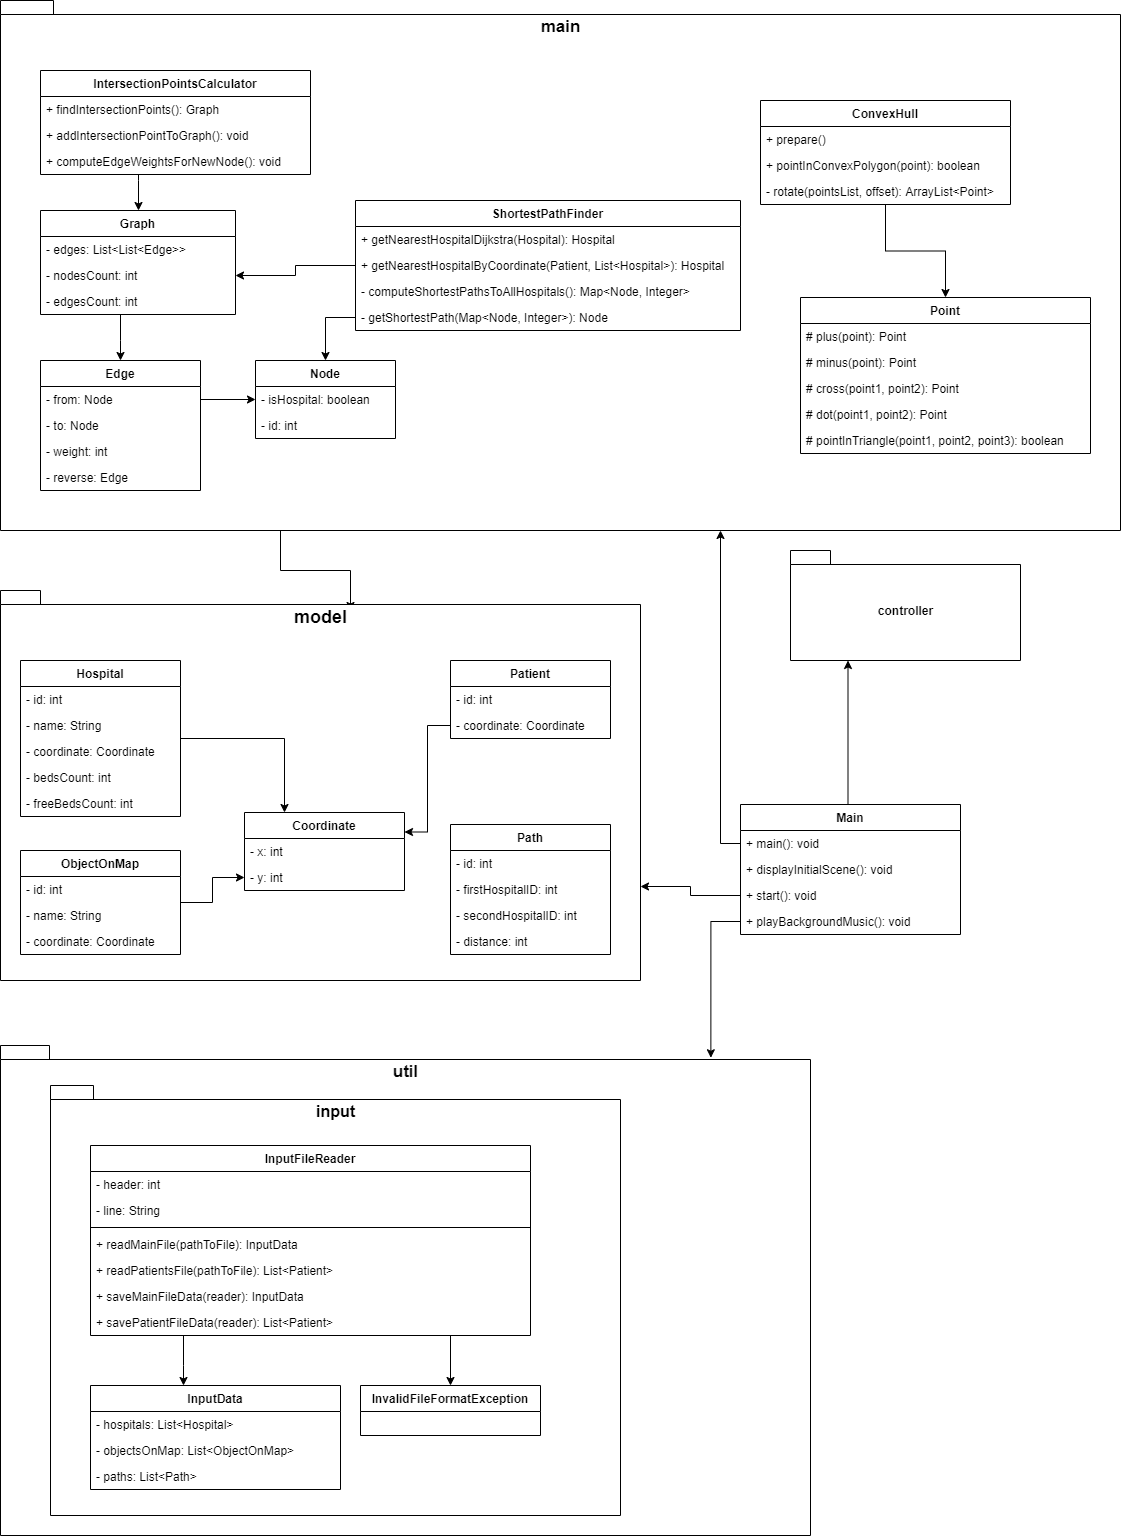
\includegraphics[width=12cm]{diagram.png}
  \caption{Diagram klas}
  \label{}
\end{figure}
\subsection{Opis klas}
\subsubsection{Pakiet model}
W tym pakiecie znajdują się klasy odpowiadające danym z pliku:\\
\textbf{Hospital} -- Szpital, który posiada współrzędne, nazwę, łączną liczbę łóżek oraz liczbę zajętych łóżek.\\
\textbf{ObjectOnMap} -- obiekt na mapie, posiada współrzędne i nazwę. Służy on tylko do wyznaczania granic.\\
\textbf{Path} -- Droga pomiędzy dwoma szpitalami, ma swoje id oraz określony dystans.\\
\textbf{Patient} -- Pacjent, posiada id oraz współrzędne.\\
\subsubsection{Pakiet util}
W tym pakiecie będą znajdować się klasy pomocnicze.\\\\
Pakiet util.input:\\
Ten pakiet będzie odpowiedzialny za wczytywanie plików. \\
\textbf{InputFileReader} - klasa ta posiada metody do wczytywania pliku głównego oraz pliku z pacjentami.\\
\textbf{InputData} - w tej klasie przechowywane są dane wczytane z pliku głównego -- szpitale, drogi, obiekty. \\
\textbf{InvalidFileFormatException} -- wyjątek rzucany przez klasę InputFileReader, jeżeli format pliku nie jest poprawny. 
\subsubsection{Pakiet controller}
W tym pakiecie znajdą się klasy odpowiedzialne za zarządzanie treściami wyświetlanymi w powłoce graficznej.
\subsubsection{Pakiet main}
W tym pakiecie znajdą się klasy realizujące logikę programu z użyciem opisanych wcześniej algorytmów.\\
\textbf{IntersectionPointsCalculator} -- zadaniem tej klasy będzie obliczanie skrzyżowań, ich położenia oraz odległości między nimi a szpitalami, które wyznaczają przecinające się drogi. \\
\textbf{ShortestPathFinder} -- klasa realizująca znajdowanie najkrótszej drogi, którą może pojechać karetka. Metoda getNearestHospitalByCoordinate będzie zwracała szpital, do którego powinno się zwieźć pacjenta z jego domu. W tym wypadku uwzględniane będą tylko współrzędne. Metoda getNearestHospitalDijkstra będzie zwracała szpital, który znajduje się najbliżej szpitala, w którym aktualnie znajduje się pacjent. Uwzględnione zostaną tu odległości dróg między szpitalami oraz między skrzyżowaniami.\\
\textbf{Graph, Edge, Node} -- struktura danych, z której korzystać będą klasy IntersectionPointsCalculator oraz ShortestPathFinder. Graf będzie składał się z krawędzi, których początkiem i końcem będą wierzchołki posiadające identyfikator oraz atrybut określający czy obiekt jest szpitalem.\\
\textbf{ConvexHull} - klasa obliczająca granice kraju z wykorzystaniem wyżej opisanego algorytmu. Korzysta ona z klasy Point, która reprezentuje punkt i posiada podstawowe metody umożliwiające dodawanie, odejmowanie punktów, jak i obliczanie iloczynów wektorowych i skalarnych.
\end{document}
